\begin{figure*}
  \centering
    \begin{subfigure}[c]{0.05\textwidth}
    ~
  \end{subfigure}
  % 
  \begin{subfigure}[c]{0.45\textwidth}
    \centering
    ~~\textbf{Mild plate effects}
  \end{subfigure}
  % 
  \begin{subfigure}[c]{0.45\textwidth}
    \centering
    ~~\textbf{Strong plate effects}
  \end{subfigure}

  \begin{subfigure}[c]{0.05\textwidth}
    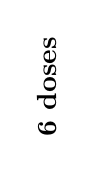
\begin{tikzpicture}
      \node[rotate=90] {\textbf{6 doses}};  
    \end{tikzpicture}
  \end{subfigure}  
  %
  \begin{subfigure}[c]{0.45\textwidth}
    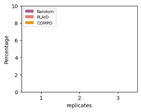
\includegraphics[width=\textwidth]{figures/percentage-low-r2-curves-1-2-3-6doses-dil18-bowl-neg-controls-0.055.png}
    %\caption{6doses-dil8-bowl-0.055}
    % \label{fig:tem}
  \end{subfigure}
  %
  \begin{subfigure}[c]{0.45\textwidth}
    \centering
    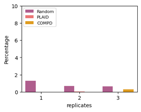
\includegraphics[width=\textwidth]{figures/percentage-low-r2-curves-1-2-3-6doses-dil18-bowl-neg-controls-0.085.png}
    %\caption{6doses-dil18-bowl-0.085}
    % \label{fig:tem}
  \end{subfigure}

  \begin{subfigure}[c]{0.05\textwidth}
    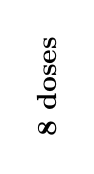
\begin{tikzpicture}
      \node[rotate=90] {\textbf{8 doses}};  
    \end{tikzpicture}
  \end{subfigure}  
  %
  \begin{subfigure}[c]{0.45\textwidth}
    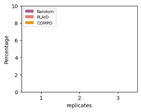
\includegraphics[width=\textwidth]{figures/percentage-low-r2-curves-1-2-3-8doses-dil8-bowl-neg-controls-0.055.png}
    %\caption{8doses-dil8-bowl-0.055}
    % \label{fig:tem}
  \end{subfigure} 
  %
  \begin{subfigure}[c]{0.45\textwidth}
    \centering
    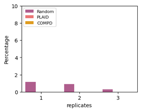
\includegraphics[width=\textwidth]{figures/percentage-low-r2-curves-1-2-3-8doses-dil8-bowl-neg-controls-0.085.png}
    %\caption{8doses-dil8-bowl-0.085}
    % \label{fig:tem}
  \end{subfigure}

  \begin{subfigure}[c]{0.05\textwidth}
    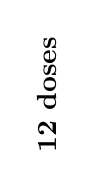
\begin{tikzpicture}
      \node[rotate=90] {\textbf{12 doses}};  
    \end{tikzpicture}
  \end{subfigure}  
  %
   \begin{subfigure}[c]{0.45\textwidth}
    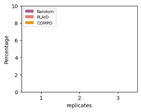
\includegraphics[width=\textwidth]{figures/percentage-low-r2-curves-1-2-3-12doses-dil4-bowl-neg-controls-0.055.png}
    %\caption{12doses-dil4-bowl-0.055}
    % \label{fig:tem}
  \end{subfigure} 
  %
  \begin{subfigure}[c]{0.45\textwidth}
    \centering
    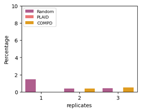
\includegraphics[width=\textwidth]{figures/percentage-low-r2-curves-1-2-3-12doses-dil4-bowl-neg-controls-0.085.png}
    %\caption{Residuals 12doses-dil4-bowl-0.085}
    % \label{fig:tem}
  \end{subfigure}
  \caption{Percentage of dose-response curves with low-quality
    ($R^2 < 80\%$) using various numbers of doses, replicates, and
    bowl-shaped plate-effect strengths. The 4PL sigmoide curves were
    fitted using compound data and 4 negative controls such that their
    mean was equal to the mean of the 20 negative controls the plate.}
\end{figure*}



%%% Local Variables: 
%%% mode: latex
%%% TeX-master: "supplement.tex"
%%% End: 